% !TEX root = ../../presentation.tex
% Core

\begin{slide}{conversions}
  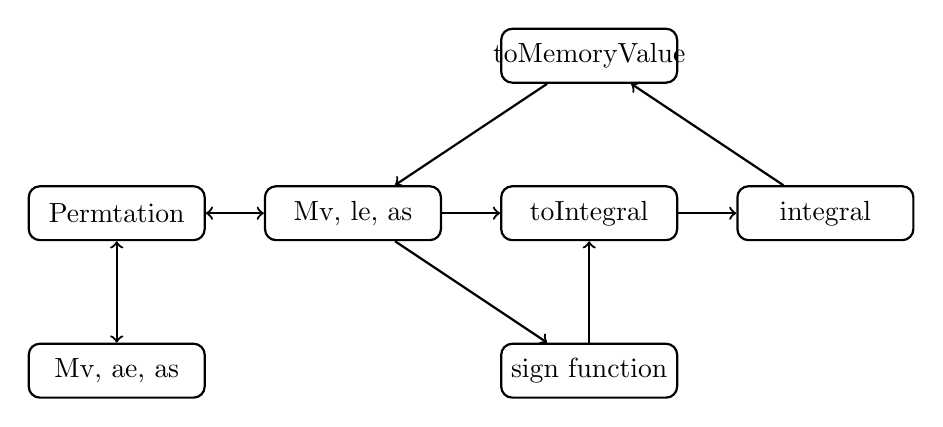
\begin{tikzpicture}[thick]

    \tikzset{block/.style={%
      draw,%
      rectangle,%
      rounded corners,%
      text width=2cm,%
      text height=0.45cm}%
    };

    \tikzset{smallblock/.style={block, text width=1.5cm, text height=0.3cm}};

    %%%%%%%%%%%%%%%
    % conversions %
    %%%%%%%%%%%%%%%
    \path (-9, -1.8) coordinate [block] (mvae) node {Mv, ae, as};

    \path (-9, 0.2) coordinate [block] (perm) node {Permtation};

    \path (-6, 0.2) coordinate [block] (mvle) node {Mv, le, as};

    \path (-3, -1.8) coordinate [block] (sf) node {sign function};

    \path (-3, 0.2) coordinate [block] (ti) node {toIntegral};

    \path (-3, 2.2) coordinate [block] (tmv) node {toMemoryValue};

    \path (0, 0.2) coordinate [block] (inte) node {integral};

    \draw [<->] (mvae) -- (perm);
    \draw [<->] (perm) -- (mvle);
    \draw [->] (mvle) -- (sf);
    \draw [->] (mvle) -- (ti);
    \draw [->] (sf) -- (ti);
    \draw [->] (ti) -- (inte);
    \draw [->] (inte) -- (tmv);
    \draw [->] (tmv) -- (mvle);

  \end{tikzpicture}
\end{slide}

\begin{slide}{register}
  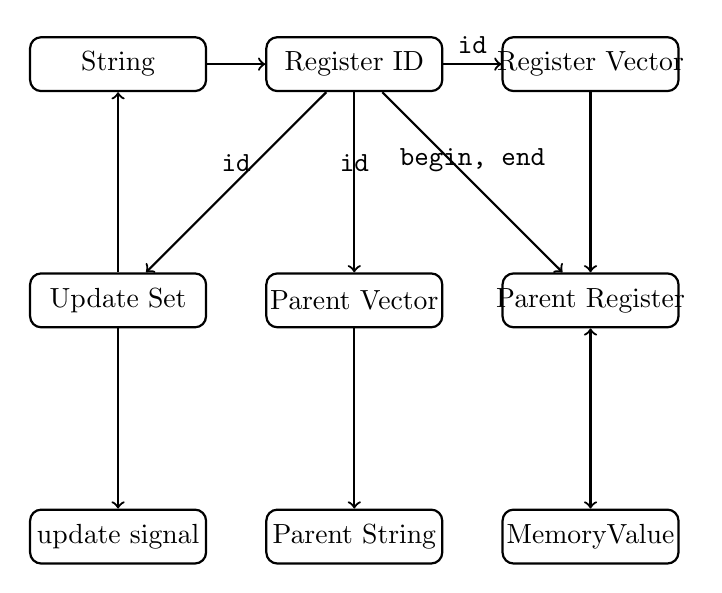
\begin{tikzpicture}[thick]

    \tikzset{block/.style={%
      draw,%
      rectangle,%
      rounded corners,%
      text width=2cm,%
      text height=0.45cm}%
    };

    \tikzset{smallblock/.style={block, text width=1.5cm, text height=0.3cm}};

    %%%%%%%%%%%%%%%
    %  register   %
    %%%%%%%%%%%%%%%
    \path (-3, 3) coordinate [block] (str) node {String};
    \path (0, 3) coordinate [block] (rid) node {Register ID};
    \path (3, 3) coordinate [block] (rvc) node {Register Vector};
    \path (3, 0) coordinate [block] (pre) node {Parent Register};
    \path (3, -3) coordinate [block] (mvl) node {MemoryValue};
    \path (-3, 0) coordinate [block] (ups) node {Update Set};
    \path (0, 0) coordinate [block] (pvc) node {Parent Vector};
    \path (0, -3) coordinate [block] (pst) node {Parent String};
    \path (-3, -3) coordinate [block] (sig) node {update signal};

    \draw [->] (str) -- (rid);
    \draw [->] (rid) -- (rvc) node [midway, above] {\texttt{id}};
    \draw [->] (rvc) -- (pre);
    \draw [->] (rid) -- (pre) node [midway, above] {\texttt{begin, end}};
    \draw [<->] (pre) -- (mvl);
    \draw [->] (rid) -- (ups) node [midway, above] {\texttt{id}};
    \draw [->] (ups) -- (str);
    \draw [->] (rid) -- (pvc) node [midway, above] {\texttt{id}};
    \draw [->] (pvc) -- (pst);
    \draw [->] (ups) -- (sig);

  \end{tikzpicture}
\end{slide}

\begin{slide}{MemoryValue}
  \begin{tabular}{l|cccc}
    x & rw-single-bit & rw-single-byte & rw-subString & constructionTime-size \\
    std::vector\textless bool\textgreater & v & x & v & v \\
    boost::dynamic\_bitset & v & x & x & v \\
    std::bitset & v & x & x & x \\
    std::vector\textless std::uint8\_t\textgreater & x & v & v & v \\
    magic & v & v & v & v \\
  \end{tabular}
\end{slide}
